\section{High Speed Elektronik}
\subsection{Serial Data Communication}
\begin{compactitem}
    \item Die maximale Übertragungsgrenze im Kupfer beträgt 12 GHz.
    \item Die Übertragungsgrenze für einen Parallelbus liegt bei 1 GHz.
\end{compactitem}

\begin{wrapfigure}[6]{r}{0.5\textwidth}
    %\vspace{-12pt}
    \centering
    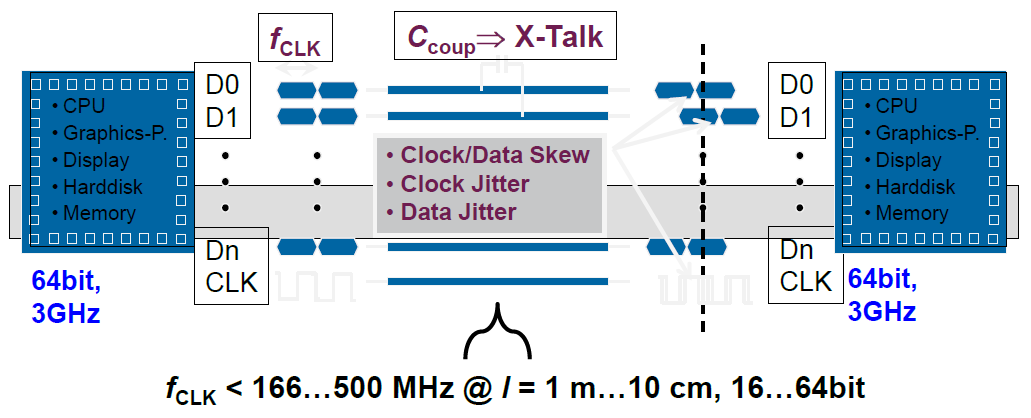
\includegraphics[width=0.45\textwidth]{images/parallel_bottleneck}
\end{wrapfigure}
\ 
\vspace{-5pt}
\subsubsection{Parallel I/O Bottleneck}
\begin{compactitem}
    \item Internal throughput: 24 GB/s
    \item I/O throughput: 1…4 GB/(s*m)
\end{compactitem}
\ \\

\subsection{High Speed Wandler Interfaces}
\subsubsection{Probleme}
Die schnellsten ADCs haben heute Abtastraten bis Gsa/sec. Das Maximum heute ist 12 Bit Auflösung bei 4GS/s. Dies ergibt eine Datenrate von 48GB/s. Ein I2C oder SPI-Interface kann die Daten nicht abholen. Auch ein Parallel-Interface ist zu langsam. Aus diesem Grund sind andere Lösungen gefragt.

\begin{multicols}{2}
    \subsubsection{Parallel CMOS or LVDS Interfaces}
    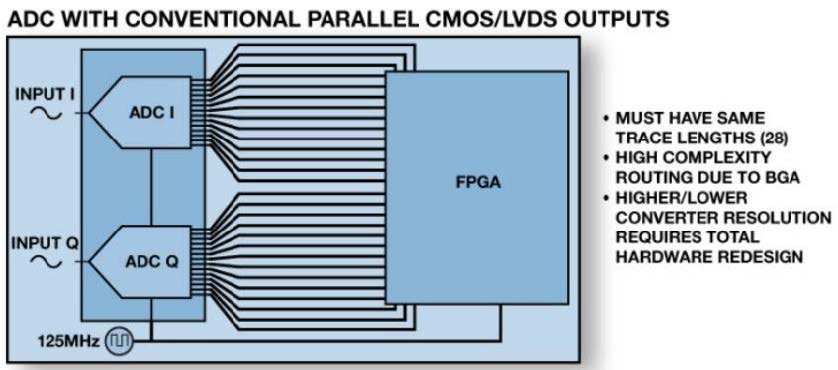
\includegraphics[width=0.45\textwidth]{images/adc_conventional}

    \subsubsection{JESD204B Interface}
    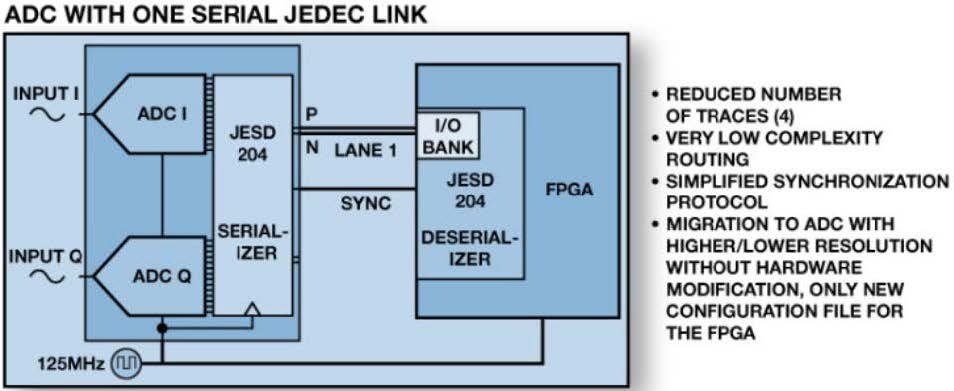
\includegraphics[width=0.48\textwidth]{images/adc_jesd}
\end{multicols}
Standard CMOS Logik ist bei hohen Datenraten nicht mehr sparsam. LVDS und auch CML sind besser geeignet. JESD204 verwendet CML.

\subsubsection{JESD204B: Input/Output}
Der Aus- und Eingang enthalten je einen 50 Ohm Abschluss.

\subsection{Programmierbare Logik}
\begin{wrapfigure}[10]{l}{0.46\textwidth}
    \hspace{-60pt}
    \centering
    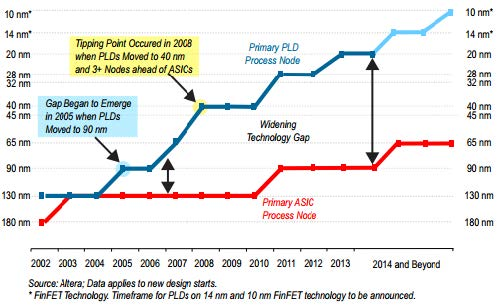
\includegraphics[width=0.45\textwidth]{images/fpga_technology}
\end{wrapfigure}
\subsubsection{Trend}
Vor 10-20 Jahren gab es noch diverse Hersteller. Diverse CPLD und FPGA-Hersteller sind mittlerweile ausgestiegen. \\
Der Highest Speed ist bald erreicht mit Silizium-ICs. Die Preise für ICs sind dabei exorbitant. Ebenfalls ist der Markt für Anwendungen mit maximalem Speed beschränkt. \\
\ \\ \ \\ \ \\ \ \\

\begin{wrapfigure}[7]{l}{0.31\textwidth}
    \hspace{-60pt}
    \centering
    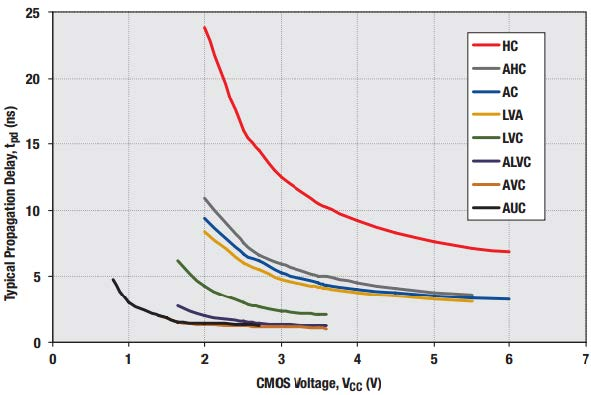
\includegraphics[width=0.28\textwidth]{images/cmos_logic}
\end{wrapfigure}
\subsection{CMOS-Logik}
\begin{compactitem}
    \item State of the art für integrierte Bausteine.
    \item Kein statischer Stromverbrauch.
    \item Aber: dynamischer Stromverbrauch steigt mit Frequenz.
    \item Logik-Pegel: 30\%  und 70\%  von VDD
    \item Schalt-Schwelle meistens nahe bei 50\%
    \item Entweder leitender Pfad nach VSS (mit NMOS) oder VDD (mit PMOS)
\end{compactitem}

\clearpage
\newpage

\subsection{TTL Transistor-Transistor-Logik}
\begin{compactitem}
    \item Transistor besteht aus 2 Dioden (BE und BC).
    \item Wegen hohem bf (Stromverstärkung im Vorwärtsbetrieb) wird Abschalten beschleunigt.
    \item Eingangssignal auf Emitter.
    \item Statischer Stromverbrauch.
    \item Komplexere Schaltungen.
    \item Aber: Bipolar ist schneller als MOS.
\end{compactitem}

\subsection{High-Speed-Logik}
\begin{compactitem}
    \item Vollständiges Ein-und Ausschalten von Transistoren ist langsam.
    \item Grosser Spannungshub bei CMOS, TTL (Grössere Ströme nötig (für gleiche Kapazitäten)).
    \item Ansatz: Kein vollständiges On/Off der Transistoren, Reduzierter Spannungshub, Stromsteuerung: Ströme können schneller geschaltet werden als Spannungen
\end{compactitem}

\begin{multicols}{2}
    \subsubsection{PECL}
    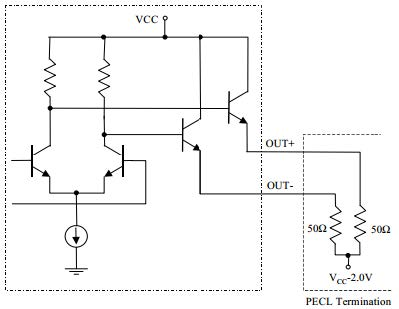
\includegraphics[width=0.35\textwidth]{images/pecl}
    \begin{compactitem}
        \item ECL 100K Serie ist schneller als 10K
        \item 50 Ohm Abschluss zu VCC-2V nötig
    \end{compactitem}
    
    \subsubsection{CML}
    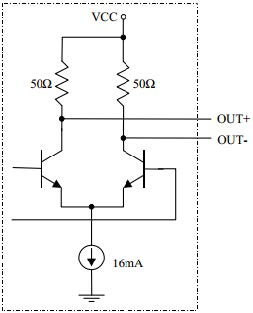
\includegraphics[width=0.20\textwidth]{images/cml}
    \begin{compactitem}
        \item Wegen Reflexionsdämpfung sollte der Ausgang mit 50 Ohm abgeschlossen werden
        \item Damit wird differentieller Pegel: +/-400mV
        \item Neuere CML-Variante: Common Mode um 1V: Geschwindigkeiten von 6.375 Gb/s bis 12.5 Gb/s
    \end{compactitem}
\end{multicols}

\subsubsection{LVDS: Low voltage differential signaling}
\begin{multicols}{2}
    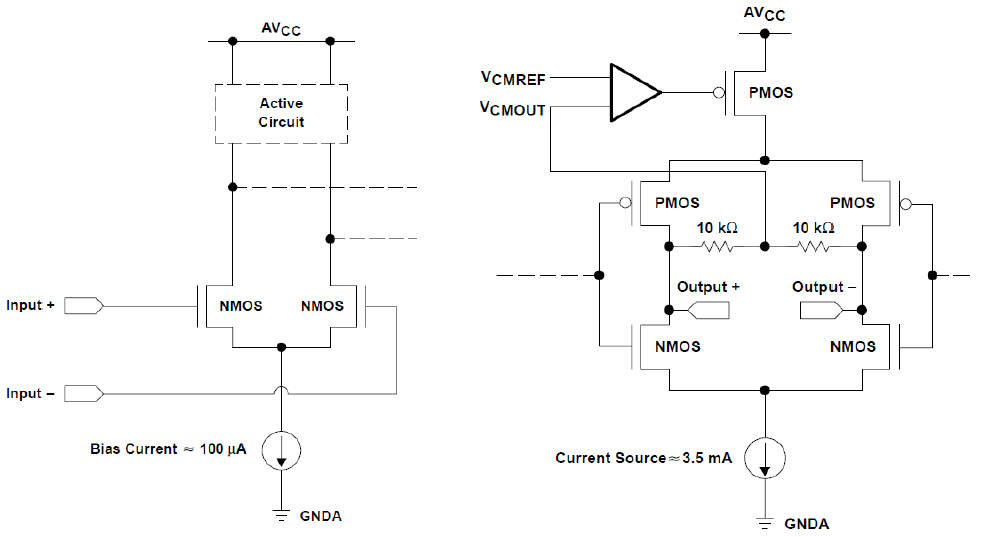
\includegraphics[width=0.48\textwidth]{images/lvds}
    \begin{compactitem}
        \item LVDS wird mehrheitlich mit CMOS implementiert.
        \item Der Ausgangsstrom beträgt 3.5 mA.
        \item LVDS muss differentiell abgeschlossen werden mit 100 Ohm.
        \item Datenraten bis 655 Mb/s sind möglich
    \end{compactitem}
\end{multicols}

\subsection{Leitungstheorie}
\subsubsection{Probleme}
\begin{compactitem}
    \item Leitungen haben Widerstände, Kapazitäten und Induktivitäten.
    \item Fortpflanzungsgeschwindigkeit Signal ~10cm-20cm/ns (Lichtgeschwindigkeit 30cm/ns)
    \item Leitungen werden zu komplexen Gebilden.
    \item Hochfrequente Signale werden reflektiert. Reflexionen entstehen, wenn Quellen-Kabel-und Lastimpedanzen nicht identisch sind.
\end{compactitem}

\subsubsection{Verbesserungen}
\begin{compactitem}
    \item Differentielle Logik erhöht Störabstand. Dadurch sind tiefere Pegelunterschiede möglich bei gleicher Zuverlässigkeit.
    \item Reduktion der Reflexion durch Terminierung der Leitung.
    \item Niederohmige Leitungen verwenden.
    \item Die meistverwendete Impedanz ist: 50 Ohm (z.B. BNC-Kabel)
\end{compactitem}